\documentclass[border=3pt]{standalone}
\usepackage[T1]{fontenc}\usepackage{mathptmx}\usepackage{amsmath,amssymb}\usepackage{tikz}
\usetikzlibrary{positioning,fit,arrows.meta,calc,backgrounds}
\begin{document}
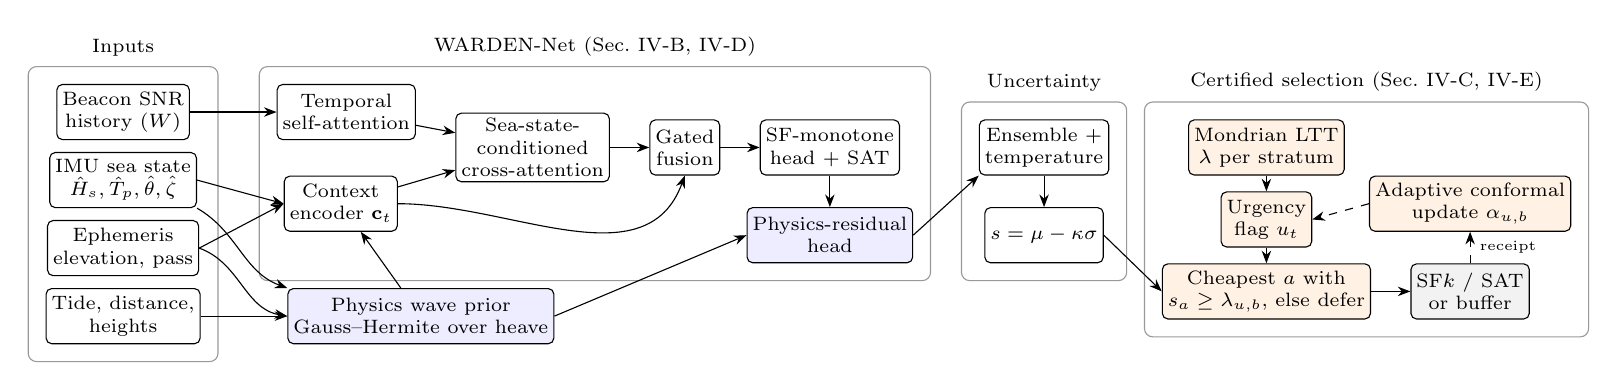
\begin{tikzpicture}[font=\scriptsize, node distance=3mm and 4mm,
  b/.style={draw, rounded corners=2pt, align=center, inner sep=2pt, minimum height=7mm, fill=white},
  phys/.style={b, fill=blue!7}, sel/.style={b, fill=orange!10},
  grp/.style={draw=black!40, rounded corners=3pt, inner sep=2.2mm},
  >={Stealth[length=1.6mm]}]
\node[b] (snr) {Beacon SNR\\history ($W$)};
\node[b, below=1.5mm of snr] (imu) {IMU sea state\\$\hat H_s,\hat T_p,\hat\theta,\hat\zeta$};
\node[b, below=1.5mm of imu] (eph) {Ephemeris\\elevation, pass};
\node[b, below=1.5mm of eph] (geo) {Tide, distance,\\heights};
\node[b, right=11mm of snr] (sa) {Temporal\\self-attention};
\node[b, right=11mm of imu, yshift=-3mm] (ctx) {Context\\encoder $\mathbf{c}_t$};
\node[phys, right=11mm of geo] (prior) {Physics wave prior\\Gauss--Hermite over heave};
\node[b, right=5mm of sa, yshift=-4.5mm] (xa) {Sea-state-\\conditioned\\cross-attention};
\node[b, right=5mm of xa] (gf) {Gated\\fusion};
\node[b, right=5mm of gf] (head) {SF-monotone\\head $+$ SAT};
\node[phys, below=4mm of head] (res) {Physics-residual\\head};
\node[b, right=10mm of head] (ens) {Ensemble $+$\\temperature};
\node[b, below=4mm of ens] (score) {$s=\mu-\kappa\sigma$};
\node[sel, right=10mm of ens] (ltt) {Mondrian LTT\\$\lambda$ per stratum};
\node[sel, below=2mm of ltt] (urg) {Urgency\\flag $u_t$};
\node[sel, below=2mm of urg] (rule) {Cheapest $a$ with\\$s_a\ge\lambda_{u,b}$, else defer};
\node[b, fill=black!5, right=5mm of rule] (out) {SF$k$ / SAT\\or buffer};
\node[sel, above=4mm of out] (aci) {Adaptive conformal\\update $\alpha_{u,b}$};
\begin{scope}[on background layer]
\node[grp, fit=(snr)(geo), label={[font=\scriptsize]above:Inputs}] {};
\node[grp, fit=(sa)(ctx)(xa)(gf)(head)(res), label={[font=\scriptsize]above:WARDEN-Net (Sec.~IV-B, IV-D)}] {};
\node[grp, fit=(ens)(score), label={[font=\scriptsize]above:Uncertainty}] {};
\node[grp, fit=(ltt)(rule)(out)(aci), label={[font=\scriptsize]above:Certified selection (Sec.~IV-C, IV-E)}] {};
\end{scope}
\draw[->] (snr) -- (sa); \draw[->] (imu.east) -- (ctx.west); \draw[->] (eph.east) -- (ctx.west);
\draw[->] (geo) -- (prior); \draw[->] (imu.south east) to[out=-30,in=160] (prior.north west); \draw[->] (eph.east) to[out=-20,in=170] (prior.west);
\draw[->] (prior) -- (ctx); \draw[->] (sa) -- (xa); \draw[->] (ctx) -- (xa); \draw[->] (xa) -- (gf);
\draw[->] (ctx.east) to[out=0,in=-110] (gf.south); \draw[->] (gf) -- (head); \draw[->] (head) -- (res);
\draw[->] (prior.east) -- (res.west); \draw[->] (res.east) -- (ens.south west); \draw[->] (ens) -- (score);
\draw[->] (score.east) -- (rule.west); \draw[->] (ltt) -- (urg); \draw[->] (urg) -- (rule); \draw[->] (rule) -- (out);
\draw[->, dashed] (out) -- node[right, font=\tiny]{receipt} (aci); \draw[->, dashed] (aci.west) -- (urg.east);
\end{tikzpicture}
\end{document}
